\documentclass[twocolumn,a4paper,11pt]{scrartcl}

% Language and font encoding
\usepackage[spanish,es-noshorthands]{babel}
\usepackage[utf8]{inputenc}
\usepackage[T1]{fontenc}

% Other necessary packages
\usepackage{graphicx}
\usepackage{amsmath}
\usepackage{cite}

\usepackage{url}
\usepackage{hyperref}

% Additional formatting for two-column layout with centered abstract
\renewcommand{\absnamepos}{empty}  % Remove space where "Abstract" title was
\addto{\captionsspanish}{\renewcommand{\abstractname}{}} % quitar título del resumen

% Title information
\title{Vida Media del Muón}
\author{Brian D. Leiva. ECFM-USAC}
\date{Mayo 2025}

\begin{document}

\twocolumn[
  \begin{@twocolumnfalse}
    \maketitle
    \begin{abstract}
      \begin{center}
      \begin{minipage}{0.6\textwidth}
  En esta práctica se determinó experimentalmente la vida media del muón a partir del análisis de datos recolectados en un detector de radiación Cherenkov. Se procesaron archivos de datos PAA para identificar pulsos con picos dobles, permitiendo la construcción de un histograma de tiempos de decaimiento.  Se aplicó un ajuste exponencial a los datos del histograma, obteniendo una vida media de  $\tau = 2.18 \pm 0.2 \mu s$, valor consistente con el valor aceptado de $2.20 \mu s$.
  \end{minipage}
  \end{center}
  \end{abstract}
\end{@twocolumnfalse}
]

\section{Objetivos}
En esta práctica tenemos como objetivo la verificación del tiempo de vida media del muón basándonos en datos experimentales obtenidos por medio de un detector de radiación Cherenkov.

\section{Marco teórico}

\subsection*{Muón}
El muón ($\mu^-$) es una partícula elemental perteneciente a la familia de los leptones, similar al electrón pero mucho más masivo (aproximadamente 207 veces la masa del electrón). Como el electrón, posee carga eléctrica negativa y espín 1/2 \cite{Martin2010} \cite{WikipediaMuon}. Al ser inestable, el muón se desintegra a través de la interacción débil, decayendo principalmente en un electrón, un antineutrino electrónico y un neutrino muónico.  Su existencia fue predicha por Fermi en 1934 y experimentalmente detectada en 1936 por Carl D. Anderson.

\subsection*{Vida Media}
La vida media ($\tau$) es el tiempo característico que tarda una población de partículas inestables en reducirse a la mitad debido a su desintegración. Para una muestra inicial de N partículas, la ley de desintegración radiactiva se describe mediante la ecuación:
\begin{equation}
  \label{eq:exponencial}
  N(t) = N_0 e^{- \lambda t }
\end{equation}

Donde:
\begin{itemize}
\item   $N(t)$ es el número de partículas presentes en el tiempo $t$.
\item   $N_0$ es el número inicial de partículas.
\item   $\lambda$ es la constante de desintegración.
\end{itemize}


\subsection*{Radiación Cherenkov}
La radiación Cherenkov es una radiación electromagnética emitida por una partícula cargada cuando se mueve a través de un medio dieléctrico a una velocidad mayor que la velocidad de la luz en ese medio. Esto ocurre porque la velocidad de la luz en un medio es menor que la velocidad de la luz en el vacío. La radiación tiene un patrón característico similar al de una onda acústica y se detecta como un cono de luz azulada \cite{WikipediaCherenkov}.


\section{Diseño experimental}
Nuestros datos fueron obtenidos utilizando un tanque Cherenkov.
\subsection*{El Tanque Cherenkov}
Un tanque Cherenkov es un recipiente lleno de un líquido transparente (generalmente agua ultrapura) diseñado para detectar la radiación Cherenkov \cite{WikipediaCherenkov} emitida por partículas cargadas que viajan a velocidades superiores a la velocidad de la luz en ese medio. La longitud del tanque y las propiedades del líquido se optimizan para maximizar la probabilidad de detección de esta radiación. En este experimento, el tanque Cherenkov permite detectar los productos de la desintegración del muón. Los datos obtenidos fueron almacenados en la carpeta de datos \cite{CarpetaDatos} en archivos .paa que contienen varios miles de pulsos, cada uno de los cuales contiene puntos de datos tomados a 8 nano segundos uno del otro.

\section{Resultados y discusión}


\begin{figure}[h]
  \centering
  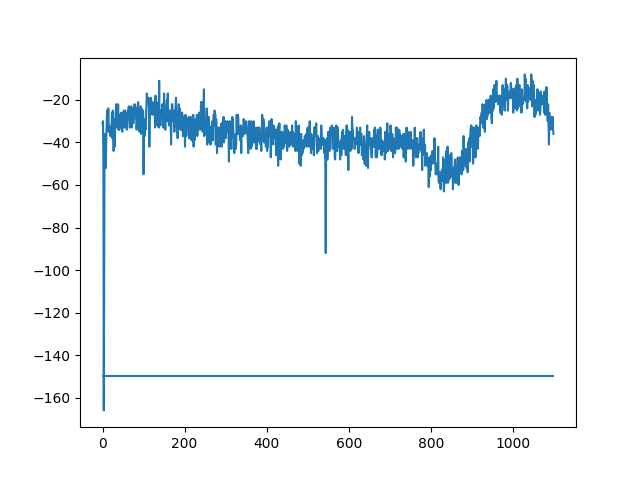
\includegraphics[width=0.5\textwidth]{pulse_plot.png}
  \caption{Ejemplo de un pulso con un pico doble.}
  \label{fig:pulse_plot}
\end{figure}

Para el procesamiento de datos partimos de los archivos .paa en la carpeta de datos \cite{CarpetaDatos} y procedimos a encontrar los pulsos con picos dobles de acuerdo al algoritmo implementado en el script vida\_media\_muon/read\_paa\_data.py del repositorio del laboratorio \cite{BrianDL_laboratorio} y descrito brevemente a continuación. 
En la figura \ref{fig:pulse_plot} se muestra un ejemplo de un pulso con un pico doble. Para encontrarlos todos recorremos cada pulso de cada archivo, y cada punto de cada uno de esos pulsos.
Al encontrar un punto que con valor menor que el umbral configurado, de -150, recorremos los puntos hasta encontrar el punto en el que la señal vuelve a incorporarse al ruido, es decir vuelve a ser mayor que -150. El pico constituye el valor máximo entre esos puntos, y lo encontramos simplemente llamando la función min() de python. Luego se configura el umbral para ser la mitad de la altura del pico ya encontrado. El tiempo de decaimiento es entonces el tiempo transcurrido entre cada par de de picos multiplicados por 8. Los tiempos de decaimiento encontrados con este proceso se pueden encontrar en el archivo vida\_media\_muon/picos\_dobles.csv en nanosegundos.

\begin{figure}[h]
  \centering
  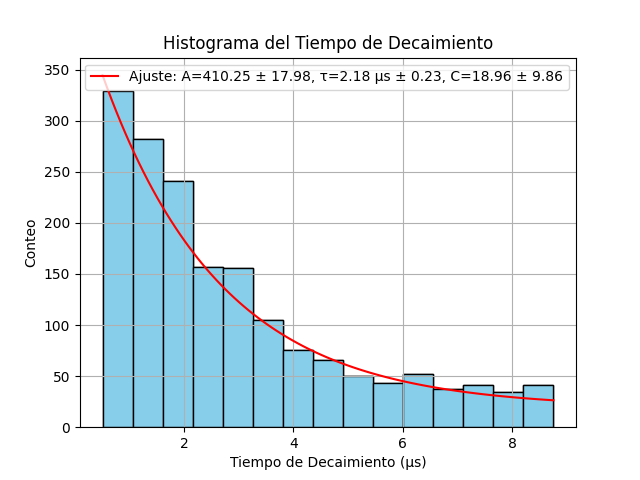
\includegraphics[width=0.5\textwidth]{histograma.png}
  \caption{Histograma de tiempos de decaimiento.}
  \label{fig:histograma}
\end{figure}

Con los datos contenidos en picos\_dobles.csv construímos un histograma (en microsegundos) al cual le realizamos un encaje lineal con la función $$Ae^{-t/\tau} + C$$ \ref{eq:exponencial} donde $\tau$ es la vida media y C es ruido de radiación de fondo que pueda afectar al sensor. El resultado se muestra en la figura \ref{fig:histograma} donde podemos ver el histograma para el cual utilizamos un binado de 15 y obtuvimos un valor para la vida media de $\tau =  2.18 \pm 0.2 \mu s$ lo cual está de acuerdo con el valor aceptado de $2.20 \mu s$. Los detalles de cómo realizar el encaje se encuenran en el script vida\_media\_muon/plot\_histogram.py.

\section{Conclusiones}

El objetivo principal de esta práctica fue determinar la vida media del muón ($\tau$) a partir de los datos recolectados en el tanque Cherenkov. Mediante el procesamiento de los archivos paa generados y la identificación de picos dobles, se construyó un histograma que permitió realizar un ajuste exponencial a los datos.

El valor obtenido para la vida media experimental fue $\tau = 2.18 \pm 0.2 \mu s$, el cual se encuentra dentro del rango del valor aceptado de $2.20 \mu s$.  Esta concordancia valida el procedimiento experimental y el análisis de datos realizado.

El método empleado es, por tanto, efectivo para la determinación de la vida media del muón y los resultados obtenidos son consistentes con las predicciones teóricas.  Las incertidumbres observadas se atribuyen principalmente a factores estadísticos y a la resolución del sistema de detección.

\bibliographystyle{ieeetr}
\bibliography{referencias} 

\end{document}